\problemname{Minequake}
\illustration{.4}{img/Goodluck_Mine.jpg}{%
  \emph{Goodluck Mine, Passage} by Ashley Dace.
  License CC BY-SA 2.0.}

\noindent
% The fully autonomous microbreweries installed in the abandoned Dwarven mines of Moravia are truly a testament to the ingenuinity and craftsmanship of Dwarven engineering!
% Alas, sometimes earthquakes rattle the mines, leading to misaligned pipes and funnels spilling precious liquid on the floor.
% As the Exalted Warden of Brewery Safety it is your responsibility to turn off the machines in every hall in case of an earthquake.
Повністю автономні мікропивоварні, встановлені в залишених копальнях карликів Моравії, дійсно свідчать про винахідливість та майстерність інженерів-карликів!
На жаль, іноді землетруси струшують копальні, що призводить до розгойдування труб та воронок, і проливання дорогоцінної рідини на підлогу.
Як на Возвеличеного Стража Безпеки Пивоварні, на Вас покладена відповідальність вимикати машини в кожному залі у випадку землетрусу.

% Walking through tunnels takes time,
% so you will inevitably arrive late at many of the machines.
% This cannot be avoided, but you want to minimise the total amount of spilled liquid.
Проходження тунелей займає час,
тому Ви невідворотно будете запізнюватися до багатьох машин.
Цього не можна уникнути, але Ви хочете мінімізувати загальну кількість розливаної рідини.

\medskip
% The Dwarven mines consist of $n$~halls connected by $n-1$~tunnels.
% The entire system is connected, so it is possible to get from any hall to any of the others.
% It takes $1$~unit of time to traverse a tunnel.
% Switching off a machines and traversing a hall takes no time.
% In each hall, turning off the machines at time~$t$ after the earthquake spills $t$~liters of liquid.
% There is exactly one earthquake, the earthquake affects all halls at the same time, and you may not switch off any machines before the earthquake.
% You can start in any of the halls.
Копальні карликів складаються з $n$ залів, що з'єднані $n-1$ тунелем.
Уся система зв'язана, тому можливо дістатися з будь-якого залу до будь-якого іншого.
Тунелі проходять за 1 одиницю часу.
Вимикання машин та проходження залів не займає часу.
У кожному залі, вимикання машин у час $t$ після землетрусу розливає $t$ літрів рідини.
Є тільки один землетрус, який впливає на всі зали одночасно, і Ви не можете вимкнути жодну машину до землетрусу.
Ви можете розпочати в будь-якому залі.

% \section*{Example}
\section*{Приклад}

% In sample input~$1$, the mines look like this:
У прикладі вхідних даних №1 копальні виглядають так:

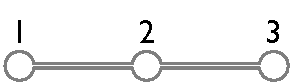
\includegraphics[width=.2\textwidth]{img/sample-1.pdf}

% If you start in hall~$2$ and visit the rest of the halls in the order $2$, $1$, $2$, $3$, then you can switch off their machines at time~$0$ (in hall $2$), time~$1$ (in hall $1$), and time~$3$ (in hall $3$).
% This wastes $0+1+3=4$~liters of liquid in total.
% If instead you start in hall~$1$ and visit the halls in the order $1$, $2$, $3$, the total amount of liquid wasted is $0+1+2=3$~liters, which is better.
Якщо Ви розпочнете з зали №2 і відвідаєте інші зали в порядку $2$, $1$, $2$, $3$, то Ви можете вимкнути їхні машини в час~$0$ (у залі $2$), час~$1$ (у залі $1$) та час~$3$ (у залі $3$).
Це зіпсує $0+1+3=4$ літрів рідини загалом.
Якщо замість цього Ви розпочнете з залу №1 і відвідаєте зали в порядку $1$, $2$, $3$, загальна кількість витраченої рідини становитиме $0+1+2=3$ літри, що краще.

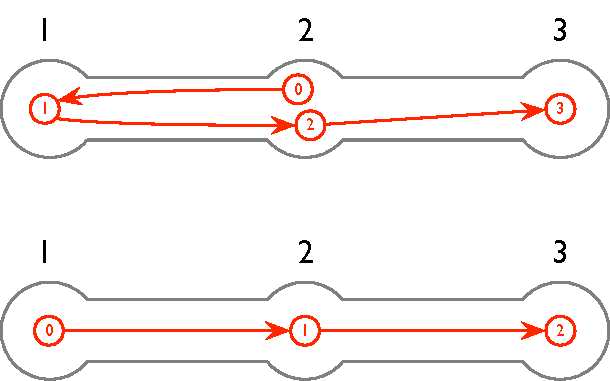
\includegraphics[width=.4\textwidth]{img/sample-1-ans.pdf}

% \section*{Input}
\section*{Вхідні дані}

% The first line of input consists of the integer $n$, denoting the number of halls.
% We assume that the halls are numbered $1$, $\ldots$, $n$.
% The next $n-1$ lines each contain two space-separated integers $u$ and $v$ with
% $1\leq u < v \leq n$, % constraint:hallnames
% meaning that there is a tunnel between hall~$u$ and hall~$v$.
Перший рядок вхідних даних містить ціле число $n$, яке позначає кількість залів.
Ми припускаємо, що зали позначені числами від $1$ до $n$.
Наступні $n-1$ рядків містять по два цілих числа $u$ та $v$ з пробілом між ними,
при цьому $1\leq u < v \leq n$, % constraint:hallnames
що означає наявність тунелю між залом $u$ та залом $v$.

% \section*{Output}
\section*{Вихідні дані}

% Print a single integer: the minimum amount of spilled liquid, in liters.
Виведіть одне ціле число: мінімальну кількість пролитої рідини в літрах.

% \section*{Constraints and Scoring}
\section*{Обмеження та оцінювання}

% We always have
% $1\leq n\leq 10^5$. % constraint:n
Ми завжди маємо:
$1\leq n\leq 10^5$. % constraint:n

% Your solution will be tested on a set of test groups, each worth a number of points.
% Each test group contains a set of test cases.
% To get the points for a test group you need to solve all test cases in the test group.
% Your final score will be the maximum score of a single submission.
Ваше рішення буде перевірено за допомогою набору тестових груп, кожна з яких оцінюється певною кількістю балів.
Кожна тестова група містить набір тестових прикладів.
Щоб отримати бали за тестову групу, необхідно успішно вирішити всі тестові приклади цієї групи.
Оцінка за завдання буде дорівнювати максимальній кількості балів, отриманій за один варіант розв'язку.

\medskip
\begin{tabular}{lll}
% Group & Points & Constraints \\\hline
Група & Бали & Обмеження \\\hline
%  $1$ & $18$ & no hall has more than two tunnels\\
  $1$ & $18$ & кожний зал має не більше двох тунелей\\
%  $2$ & $19$ & at most one hall has more than two tunnels\\
  $2$ & $19$ & не більше одного залу має більше двох тунелей\\
  $3$ & $20$ & $n\leq 10$\\
  $4$ & $21$ & $n\leq 1000$\\
%  $5$ & $22$ & \emph{No additional constraints}
  $5$ & $22$ & \emph{Немає додаткових обмежень}
\end{tabular}

